\section{Observation \& Calculation}
    \subsection{Determination of wavelength $\lambda$ of the laser light using diffraction pattern}

        Slit width b = 0.2mm and D = 4m
        \begin{table}[H]
	\centering
	\resizebox{\columnwidth}{!}{%
	\begin{tabular}{|c|c|c|c|c|c|c|c|}
	\hline
	Drop no & Sl no & \begin{tabular}[c]{@{}c@{}}Free Fall\\ time   (s)\end{tabular} & Rise time (s) & \begin{tabular}[c]{@{}c@{}}Mean Free fall\\ time\end{tabular} & \begin{tabular}[c]{@{}c@{}}Mean Rise\\ time\end{tabular} & \begin{tabular}[c]{@{}c@{}}Mean free fall velocity\\ $(v_f = \sfrac{L}{t_f}\times 10^{5})$\\ $(ms^{-1})$\end{tabular} & Voltage (V) \\ \hline
	\multirow{5}{*}{1} & 1 & 9.9 & 16.1 & \multirow{5}{*}{10.12} & \multirow{5}{*}{15.1} & \multirow{5}{*}{9.881} & \multirow{5}{*}{378} \\ \cline{2-4}
	 & 2 & 10.4 & 14.6 &  &  &  &  \\ \cline{2-4}
	 & 3 & 10.3 & 14.8 &  &  &  &  \\ \cline{2-4}
	 & 4 & 10.3 & 14.2 &  &  &  &  \\ \cline{2-4}
	 & 5 & 9.7 & 15.8 &  &  &  &  \\ \hline
	\multirow{5}{*}{2} & 1 & 8.6 & 13.7 & \multirow{5}{*}{8.56} & \multirow{5}{*}{13.84} & \multirow{5}{*}{11.682} & \multirow{5}{*}{450} \\ \cline{2-4}
	 & 2 & 8.1 & 13.9 &  &  &  &  \\ \cline{2-4}
	 & 3 & 8.7 & 14.9 &  &  &  &  \\ \cline{2-4}
	 & 4 & 9 & 13.3 &  &  &  &  \\ \cline{2-4}
	 & 5 & 8.4 & 13.4 &  &  &  &  \\ \hline
	\multirow{5}{*}{3} & 1 & 10.3 & 7 & \multirow{5}{*}{10.14} & \multirow{5}{*}{6.4} & \multirow{5}{*}{9.862} & \multirow{5}{*}{343} \\ \cline{2-4}
	 & 2 & 10 & 6.4 &  &  &  &  \\ \cline{2-4}
	 & 3 & 10.1 & 6.2 &  &  &  &  \\ \cline{2-4}
	 & 4 & 10.1 & 6.2 &  &  &  &  \\ \cline{2-4}
	 & 5 & 10.2 & 6.2 &  &  &  &  \\ \hline
	\multirow{5}{*}{4} & 1 & 11.4 & 7 & \multirow{5}{*}{11.26} & \multirow{5}{*}{6.84} & \multirow{5}{*}{8.881} & \multirow{5}{*}{500} \\ \cline{2-4}
	 & 2 & 11.2 & 6.6 &  &  &  &  \\ \cline{2-4}
	 & 3 & 11.3 & 6.8 &  &  &  &  \\ \cline{2-4}
	 & 4 & 11 & 7.1 &  &  &  &  \\ \cline{2-4}
	 & 5 & 11.4 & 6.7 &  &  &  &  \\ \hline
	\multirow{5}{*}{5} & 1 & 10.6 & 2.5 & \multirow{5}{*}{10.842} & \multirow{5}{*}{2.5} & \multirow{5}{*}{9.223} & \multirow{5}{*}{484} \\ \cline{2-4}
	 & 2 & 11.2 & 2.3 &  &  &  &  \\ \cline{2-4}
	 & 3 & 10.9 & 2.4 &  &  &  &  \\ \cline{2-4}
	 & 4 & 11.11 & 2.6 &  &  &  &  \\ \cline{2-4}
	 & 5 & 10.4 & 2.7 &  &  &  &  \\ \hline
	\multirow{5}{*}{6} & 1 & 19.7 & 8.9 & \multirow{5}{*}{19.92} & \multirow{5}{*}{8.36} & \multirow{5}{*}{5.020} & \multirow{5}{*}{400} \\ \cline{2-4}
	 & 2 & 20.4 & 7.7 &  &  &  &  \\ \cline{2-4}
	 & 3 & 18.9 & 8.3 &  &  &  &  \\ \cline{2-4}
	 & 4 & 20.4 & 8.7 &  &  &  &  \\ \cline{2-4}
	 & 5 & 20.2 & 8.2 &  &  &  &  \\ \hline
	\multirow{5}{*}{7} & 1 & 16.2 & 10.6 & \multirow{5}{*}{16.54} & \multirow{5}{*}{9.26} & \multirow{5}{*}{6.046} & \multirow{5}{*}{410} \\ \cline{2-4}
	 & 2 & 16.8 & 9.9 &  &  &  &  \\ \cline{2-4}
	 & 3 & 15.8 & 9.6 &  &  &  &  \\ \cline{2-4}
	 & 4 & 16.9 & 8.1 &  &  &  &  \\ \cline{2-4}
	 & 5 & 17 & 8.1 &  &  &  &  \\ \hline
	\end{tabular}%
	}
	\caption{Dynamic Method Data}
	\label{tab:1}
\end{table}

        \begin{figure}[H]
            \centering
            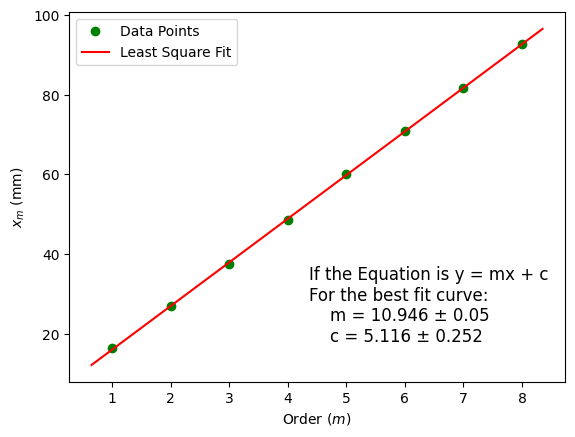
\includegraphics[width=0.5\textwidth]{images/graph_1.png}
            \caption{$x_m$ vs $m$ graph for Single Slit Diffraction}
            \label{graph:1}
        \end{figure}

        \subsubsection{Calculation \& error analysis}
            From \hyperref[graph:1]{Graph 1} we see that the slope:
            $$m\;(slope) = 10.946 mm$$
            
            
            From \hyperref[eqn:1]{Equation 1}, we know:
            
            $$m = \frac{2D\lambda}{b}$$
            $$\therefore \lambda = \frac{mb}{2D} = 656.76nm$$
            $$\delta\lambda = \lambda\sqrt{\left(\frac{\delta D}{D}\right)^2 + \left(\frac{\delta b}{b}\right)^2 + \left(\frac{\delta m}{m}\right)^2}$$
            $$\delta\lambda = 656.76\times\sqrt{400^{-2}+48^{-2}+219^{-2}}$$
            $$\delta\lambda = 14.1nm$$

            \begin{center}
                \fbox{$\lambda = 656.76\pm14.1\;nm$}
                \label{ans:1}
            \end{center}

    \subsection{Finding thickness of thin wire}
        Thickness b = 0.2mm (using travelling microscope). Distance between the wire and the screen D = 4m.



        \begin{table}[H]
	\centering
	\resizebox{\columnwidth}{!}{%
	\begin{tabular}{|c|c|c|c|c|c|c|}
	\hline
	Drop no & Sl no & \begin{tabular}[c]{@{}c@{}}Free Fall\\ time (s)\end{tabular} & \begin{tabular}[c]{@{}c@{}}Mean Free fall\\ time ($t_f$) (s)\end{tabular} & \begin{tabular}[c]{@{}c@{}}Mean free fall velocity\\ $(v_f = \sfrac{L}{t_f}$\\ $\times 10^{5}\;(ms^{-1})$\end{tabular} & Balancing voltage(V) & Voltage (V) \\ \hline
	\multirow{5}{*}{1} & 1 & 4.9 & \multirow{5}{*}{4.64} & \multirow{5}{*}{0.0002} &  & \multirow{5}{*}{238} \\ \cline{2-3} \cline{6-6}
	 & 2 & 4.6 &  &  & 238 &  \\ \cline{2-3} \cline{6-6}
	 & 3 & 4.5 &  &  & 238 &  \\ \cline{2-3} \cline{6-6}
	 & 4 & 4.4 &  &  & 238 &  \\ \cline{2-3} \cline{6-6}
	 & 5 & 4.8 &  &  & 238 &  \\ \hline
	\multirow{4}{*}{2} & 1 & 11.5 & \multirow{4}{*}{11.275} & \multirow{4}{*}{9E-05} &  & \multirow{4}{*}{306.3333} \\ \cline{2-3} \cline{6-6}
	 & 2 & 11.2 &  &  & 306 &  \\ \cline{2-3} \cline{6-6}
	 & 3 & 11.3 &  &  & 306 &  \\ \cline{2-3} \cline{6-6}
	 & 4 & 11.1 &  &  & 307 &  \\ \hline
	\multirow{4}{*}{3} & 1 & 10.6 & \multirow{4}{*}{10.125} & \multirow{4}{*}{1E-04} &  & \multirow{4}{*}{230} \\ \cline{2-3} \cline{6-6}
	 & 2 & 10.3 &  &  & 230 &  \\ \cline{2-3} \cline{6-6}
	 & 3 & 9.8 &  &  & 229 &  \\ \cline{2-3} \cline{6-6}
	 & 4 & 9.8 &  &  & 231 &  \\ \hline
	\multirow{4}{*}{4} & 1 & 15.7 & \multirow{4}{*}{15.15} & \multirow{4}{*}{7E-05} &  & \multirow{4}{*}{360} \\ \cline{2-3} \cline{6-6}
	 & 2 & 14.7 &  &  & 360 &  \\ \cline{2-3} \cline{6-6}
	 & 3 & 15.3 &  &  & 359 &  \\ \cline{2-3} \cline{6-6}
	 & 4 & 14.9 &  &  & 361 &  \\ \hline
	\multirow{4}{*}{5} & 1 & 13.6 & \multirow{4}{*}{13.525} & \multirow{4}{*}{7E-05} &  & \multirow{4}{*}{264} \\ \cline{2-3} \cline{6-6}
	 & 2 & 13.1 &  &  & 266 &  \\ \cline{2-3} \cline{6-6}
	 & 3 & 13.9 &  &  & 264 &  \\ \cline{2-3} \cline{6-6}
	 & 4 & 13.5 &  &  & 262 &  \\ \hline
	\multirow{4}{*}{6} & 1 & 13.8 & \multirow{4}{*}{13.95} & \multirow{4}{*}{7E-05} &  & \multirow{4}{*}{407.6667} \\ \cline{2-3} \cline{6-6}
	 & 2 & 14.1 &  &  & 407 &  \\ \cline{2-3} \cline{6-6}
	 & 3 & 13.7 &  &  & 409 &  \\ \cline{2-3} \cline{6-6}
	 & 4 & 14.2 &  &  & 407 &  \\ \hline
	\end{tabular}%
	}
	\caption{Balancing Method Data}
	\label{tab:2}
\end{table}

        \begin{figure}[H]
            \centering
            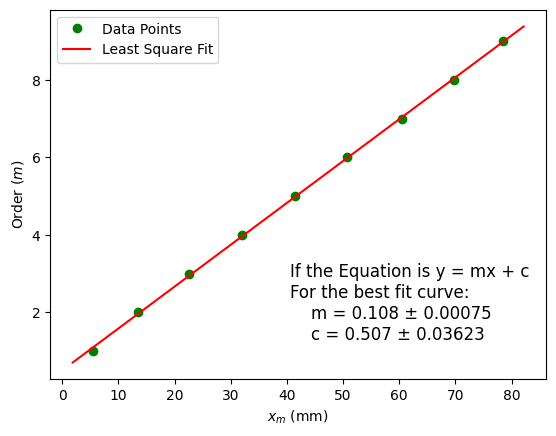
\includegraphics[width=0.5\textwidth]{images/graph_2.png}
            \caption{$m$ vs $x_m$ graph for Diffraction of thin wire}
            \label{graph:2}
        \end{figure}

        \subsubsection{Calculation \& error analysis}
            From \hyperref[graph:2]{Graph 2} we see that the slope:
            $$m\;(slope) = 0.108 mm^{-1} = 108 m^{-1}$$

            From \hyperref[eqn:2]{Equation 2}, we know:
            $$s = \frac{b}{D\lambda}$$

            For $\lambda = 656.76 nm$ (found in the \hyperref[ans:1]{last part}), we get:
            $$b = D\lambda m = 0.283mm$$
            $$\delta b = b\sqrt{\left(\frac{\delta D}{D}\right)^2 + \left(\frac{\delta \lambda}{\lambda}\right)^2 + \left(\frac{\delta m}{m}\right)^2}$$
            $$\delta b = 0.0065mm\;(2.3\%)$$

            \begin{center}
                \fbox{$\lambda = 0.283\pm0065\;mm$}
                \label{ans:2}
            \end{center}

            Error wrt to the value obtained from the travelling microscope is 29\%.

    \subsection{Verifying Babinet's Principle}
        We tried to coincide the fringes with the single slit with that obtained from the wire. Then we measured the slit width with the help of travelling microscope. We got the slit width as 0.22mm. 
        % We also calculated the slit width using the fringe pattern:
        % % Please add the following required packages to your document preamble:
% \usepackage{graphicx}
\begin{table}[H]
    \resizebox{\columnwidth}{!}{%
    \begin{tabular}{|c|c|c|c|}
    \hline
    Sl. No &
      \begin{tabular}[c]{@{}c@{}}Angular Position of\\ Analyser $(\theta)(\degree)$\end{tabular} &
      \begin{tabular}[c]{@{}c@{}}Corrected Position of\\ Analyser $(\theta)(\degree)$\end{tabular} &
      \begin{tabular}[c]{@{}c@{}}Current\\ (I) $(\mu A)$\end{tabular} \\ \hline
    1  & 6   & -104 & 165.62 \\ \hline
    2  & 20  & -90  & 222.95 \\ \hline
    3  & 30  & -80  & 248.43 \\ \hline
    4  & 50  & -60  & 286.65 \\ \hline
    5  & 70  & -40  & 261.17 \\ \hline
    6  & 90  & -20  & 203.84 \\ \hline
    7  & 110 & 0    & 133.77 \\ \hline
    8  & 130 & 20   & 70.07  \\ \hline
    9  & 140 & 30   & 50.96  \\ \hline
    10 & 150 & 40   & 44.59  \\ \hline
    11 & 154 & 44   & 50.96  \\ \hline
    12 & 160 & 50   & 57.33  \\ \hline
    13 & 170 & 60   & 76.44  \\ \hline
    14 & 190 & 80   & 133.77 \\ \hline
    15 & 220 & 110  & 235.69 \\ \hline
    16 & 250 & 140  & 261.17 \\ \hline
    17 & 270 & 160  & 273.91 \\ \hline
    18 & 276 & 166  & 267.54 \\ \hline
    19 & 290 & 180  & 203.84 \\ \hline
    20 & 300 & 190  & 159.25 \\ \hline
    21 & 320 & 210  & 89.18  \\ \hline
    22 & 330 & 220  & 108.29 \\ \hline
    \end{tabular}%
    }
    \caption{For Quarter-Wave Plate}
    \label{tab:quarter}
    \end{table}

        We find that the single slit width is approximately equal to the wire thickness (0.2mm) for an approximate pattern. This verifies Babinet's principle. (Error = 10.7\%)
    
    \subsection{Determination of the two slit widths in double slit experiment using diffraction pattern}

        From Travelling microscope:
        
        Width of first slit $(s_1) = (8.85+0.020)-(8.80+0.04) = 8.870-8.840 = 0.030cm$
        
        Width of Second slit $(s_2) = (8.90+0.008)-(8.85+0.035) = 8.908-8.885 = 0.023cm$

        $$\therefore b = \frac{0.23+0.3}{2} = 0.265mm$$
        $$\therefore d = 8.885-8.870 cm = 0.15mm$$
        $$\therefore c = 8.885-8.870 cm = 0.28mm$$

        % Please add the following required packages to your document preamble:
% \usepackage{graphicx}
\begin{table}[H]
	\centering
	\resizebox{\columnwidth}{!}{%
		\begin{tabular}{|c|c|c|c|c|}
			\hline
			\begin{tabular}[c]{@{}c@{}}pole separation\\ (mm)\end{tabular} & B (mT) & $\Delta$ & $\delta$   & $\Delta K$ \\ \hline
			40                                                             & 1900        & 5474.99  & 2749.0879  & 57.47682   \\ \hline
			42                                                             & 1700        & 5502.858 & 2209.28393 & 45.95689   \\ \hline
			44                                                             & 1050        & 5483.805 & 1769.41523 & 36.93475   \\ \hline
			45                                                             & 800         & 5349.992 & 1531.39795 & 32.76592   \\ \hline
		\end{tabular}%
	}
	\caption{B vs $\Delta K$}
	\label{tab:final}
\end{table}

        \begin{figure}[H]
            \centering
            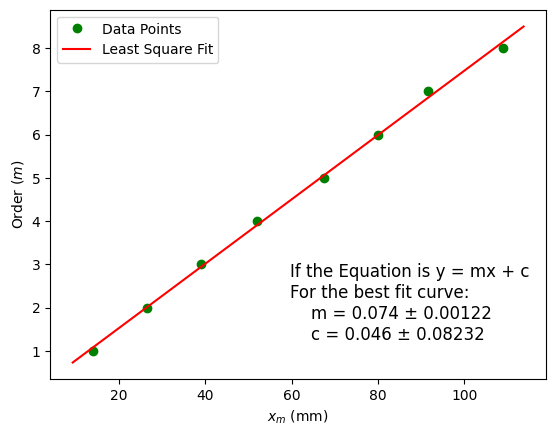
\includegraphics[width=0.4\textwidth]{images/graph_3.png}
            \caption{$m$ vs $x_m$ graph for double slit diffraction}
            \label{graph:3}
        \end{figure}

        From \hyperref[graph:3]{Graph 3} we see that the slope (m) is $0.074 mm^{-1} = 74 m^{-1}$.

        Therefore, from \hyperref[eqn:3]{Equation 3}, we get:

        $$m = \frac{b}{D\lambda}$$
        $$b = mD\lambda = 0.19mm$$


        \begin{table}[H]
	\centering
	\resizebox{\columnwidth}{!}{%
	\begin{tabular}{|ccc|c|}
	\hline
	\multicolumn{1}{|c|}{$ne\times10^{-19}$} & \multicolumn{1}{c|}{ne divided by the lowest} & $n_{eff}$ & $e = \frac{ne}{n_{eff}}$   $(\times10^{-19})$ (c) \\ \hline
	\multicolumn{1}{|c|}{6.24} & \multicolumn{1}{c|}{1.52} & 2.00 & 3.12 \\ \hline
	\multicolumn{1}{|c|}{6.59} & \multicolumn{1}{c|}{1.61} & 2.00 & 3.30 \\ \hline
	\multicolumn{1}{|c|}{10.60} & \multicolumn{1}{c|}{2.58} & 3.00 & 3.53 \\ \hline
	\multicolumn{1}{|c|}{6.32} & \multicolumn{1}{c|}{1.54} & 2.00 & 3.16 \\ \hline
	\multicolumn{1}{|c|}{13.97} & \multicolumn{1}{c|}{3.40} & 3.00 & 4.66 \\ \hline
	\multicolumn{1}{|c|}{4.10} & \multicolumn{1}{c|}{1.00} & 1.00 & 4.10 \\ \hline
	\multicolumn{1}{|c|}{4.43} & \multicolumn{1}{c|}{1.08} & 1.00 & 4.43 \\ \hline
	\multicolumn{3}{|c|}{Average value of e} & 3.76 \\ \hline
	\multicolumn{3}{|c|}{$\delta e$ (standard   deviation)} & 0.63 \\ \hline
	\end{tabular}%
	}
	\caption{Dynamic Method find value of e}
	\label{tab:5}
\end{table}

        \begin{figure}[H]
            \centering
            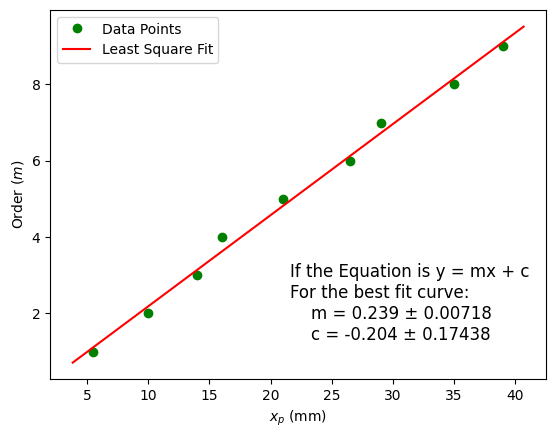
\includegraphics[width=0.5\textwidth]{images/graph_4.png}
            \caption{$m$ vs $x_p$ graph for double slit diffraction}
            \label{graph:4}
        \end{figure}

        From \hyperref[graph:4]{Graph 4} we see that the slope (m) is $0.239 mm^{-1} = 239 m^{-1}$.

        Therefore, from \hyperref[eqn:4]{Equation 4}, we get:

        $$m = \frac{d}{D\lambda}$$
        $$d = mD\lambda = 0.63mm$$

        from graph and table, $c = d-b = 0.44mm$.

        \vspace{2mm}
        The Error in the value of c when compared with the observed value with the help of travelling microscope (0.28mm) is 36.4\%.